\documentclass[12pt]{article}
\usepackage[utf8]{inputenc}
\usepackage[english]{babel}
\usepackage{url}
\usepackage{graphicx}
\usepackage{geometry}
\usepackage{hyperref}
\hypersetup{
    colorlinks=true,
    linkcolor=blue,
    filecolor=magenta,      
    urlcolor=cyan,
}
\geometry{a4paper, left=20mm, right=20mm, top=12mm, bottom=12mm}

\makeatletter         
\def\@maketitle{
\noindent\begin{minipage}{0.18\textwidth}

\includegraphics[scale=0.4]{img/wits.jpg}
\end{minipage}%
\begin{minipage}{0.9\textwidth}
\raggedright{\large\bfseries\@title}\par\medskip
\normalsize \@author \\
\small \@date
\end{minipage}
\hrule
\vspace{0.5em}}
\makeatother

\begin{document}

\title{ A Parallel Distributed Computational Pipeline \\ for maxT Permutation Testing in GWAS
}
\author{Tinozivashe Sibanda and Andisani Nemavhola}

\maketitle
\begin{abstract}
This report describes the capstone project for COMS7057A - Large Scale Computing Systems and Scientific Programming at the University of the Witwatersrand. The code can be found at the github repository for this project by visiting:  \href{next-gwas}{https://github.com/tino-sibanda/next-gwas.git}
\end{abstract}

\section{Introduction}

Genome Wide Association Studies (GWAS) look for variances in DNA sequences that occur more frequently in people with a certain disease (i.e. cases) than in people without the disease (i.e. controls)\cite{Chang2018} by comparing the frequency of alleles at each loci, usually taken as single-nucleotide polymorphisms (SNPs) \cite{Dickhaus2012}. Essentially, association testing is done per SNP using the $\chi^2$ test for independence under the null hypothesis of no association; p-values are derived from the underlying contingency table. Typically, because millions of SNPs need to be tested - causing inflated Family‐Wise Error Rates (FWER) amongst other issues, the obtained p-values are adjusted via Bonferroni correction \cite{Sethuraman2019}.\\

\noindent
Permutation testing methods are an alternative and handle FWER well, despite being computationally expensive. In particular, maxT based permutation corrects the p-values by simulating the null distribution through permuting the phenotype values (\emph{ i.e. case or control}) \cite{Goeman2014};  adjusted p-values are then calculated using the single step max-t procedure \cite{Steiss2012}.
 
\subsection{Problem Statement}
The objective of this project is to design a parallel distributed computational pipeline which performs maxT based permutation testing for association studies. From our perspective the pipeline should be portable and analytical results should be reproducible.

\subsection{Solution Approach}
The solution chosen in this project was to build a computational pipeline using \href{https://www.nextflow.io}{Nextflow} to orchestrate statistical computations written using the \href{http://zzz.bwh.harvard.edu/plink/}{Plink} tool for genome association analysis; Python functions were written to visualise the manhattan plots and qqplots.\\ 

Essentially, in this approach, blocks of 100 SNPs each are extracted and processed in parallel across different nodes on the cluster and the results are then merged together. The pipeline is available on Github at \href{https://github.com/tino-sibanda/next-gwas.git}{https://github.com/tino-sibanda/next-gwas.git}.

\subsection{Hardware}

The Wits Core Cluster (ZA-WITS-CORE) was used to run the parallel distributed pipeline. The cluster runs CentOS 7.5 and provided upto 45 worker nodes, 1000 hyper-threaded cores and, between 24GB-1TB of RAM. This cluster is setup to use \href{https://slurm.schedmd.com/}{slurm} as the job scheduling system and does not support containerization using \href{https://www.docker.com/}{Docker}.
\newpage

\section{Results and Discussion}

\subsection{Statistical Analysis}
Figure 1 below shows the Manhattan plot (left) and the qqplot (right) generated from 100 000 permutation tests. \\

The Manhattan plot shows on the y-axis the negative log-base-10 of the P value for each of the SNPs in the genome (along the x-axis), when tested for differences in frequency between 56 cases and 56 controls across 1 457 897 variants/SNPs. The line shows the threshold for genome-wide significance ($P<5 \times 10^{-8}$).

\begin{figure}[h!]
    \centering
    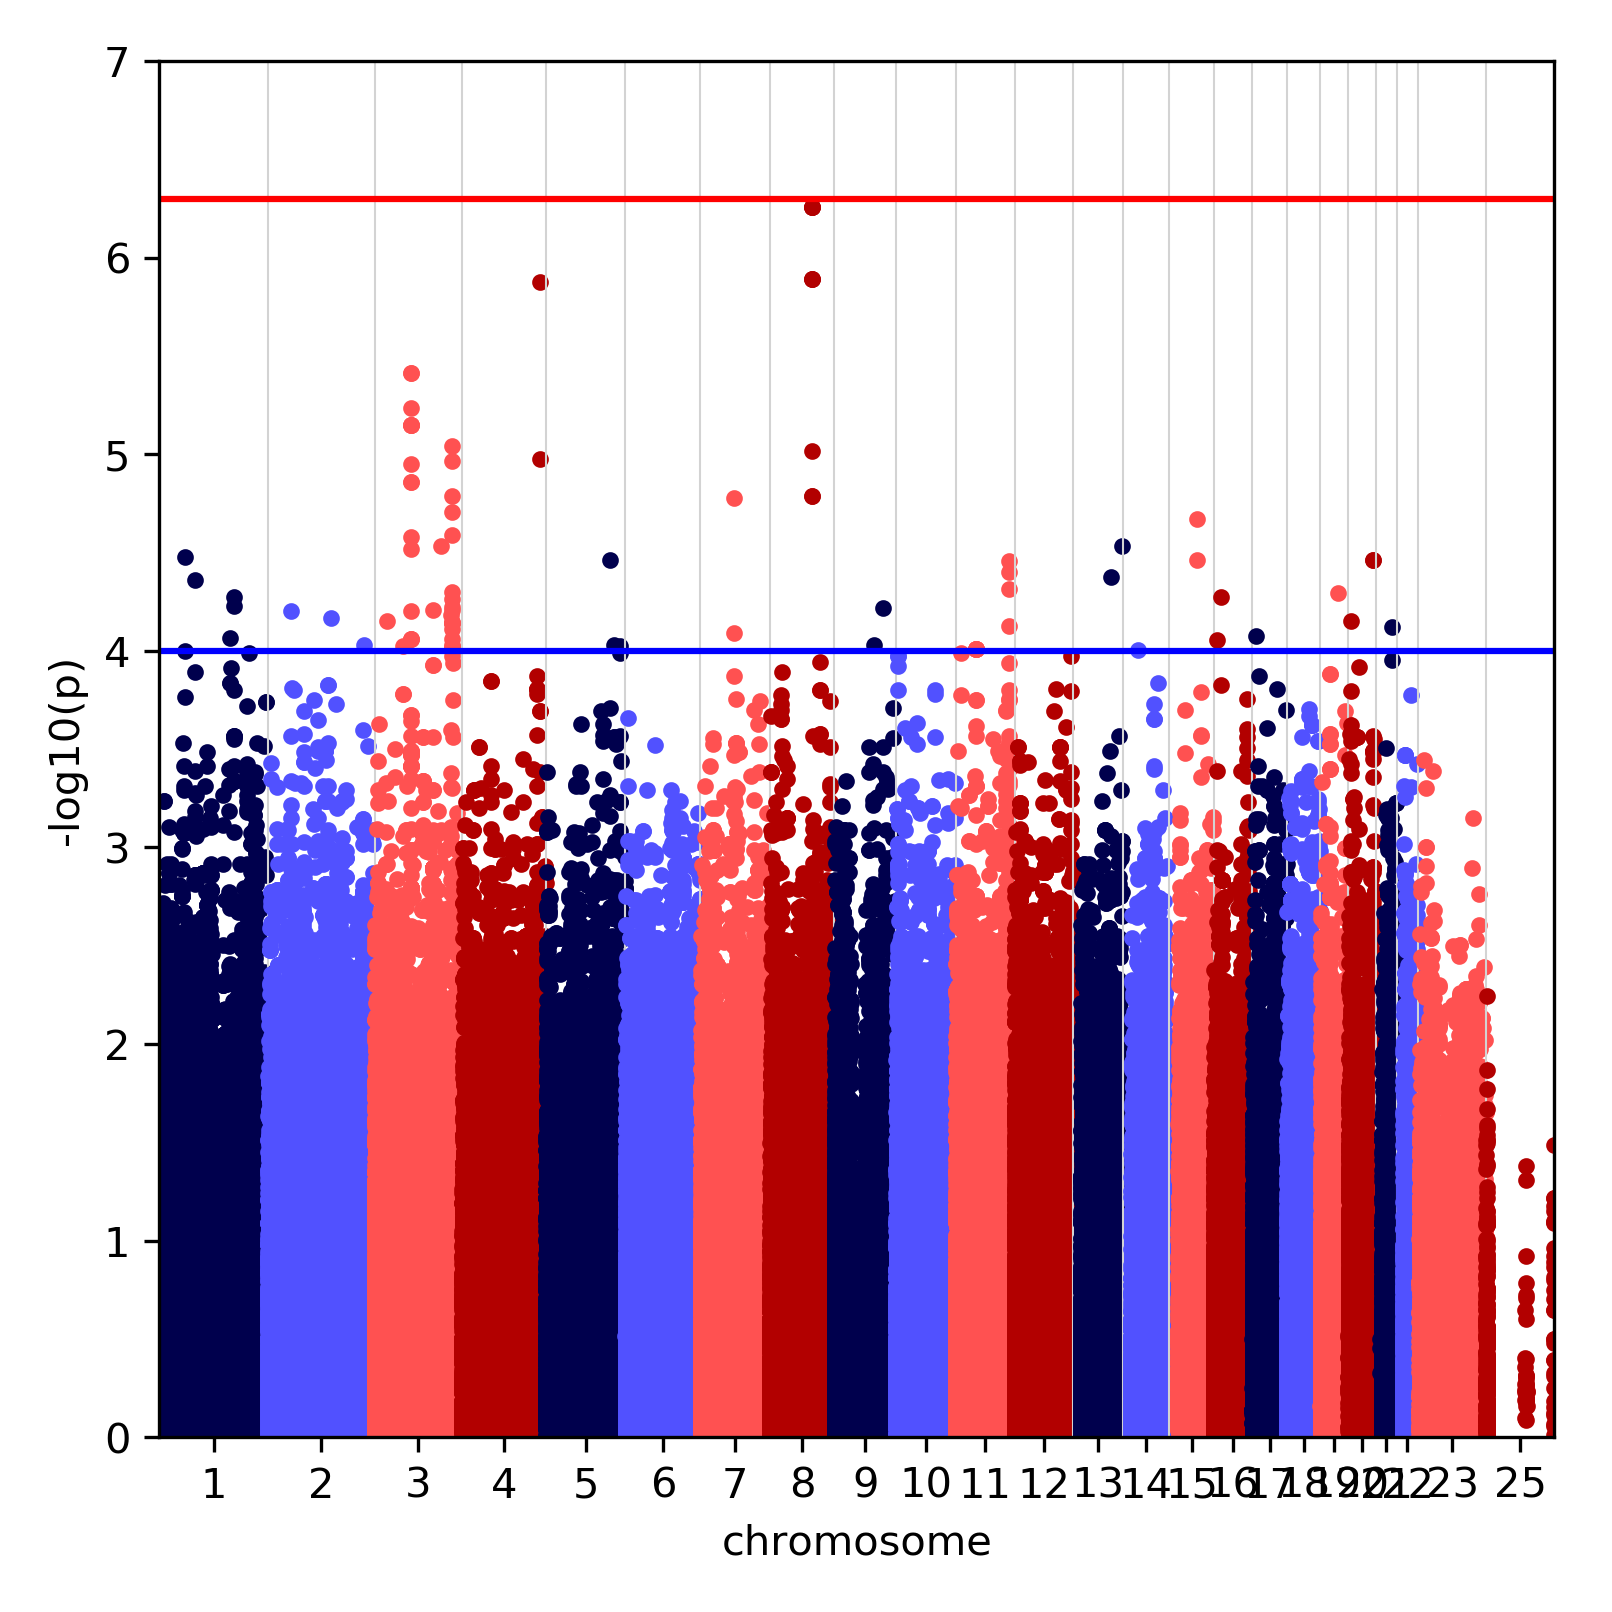
\includegraphics[scale=0.5]{img/manhattan_plot.png}
    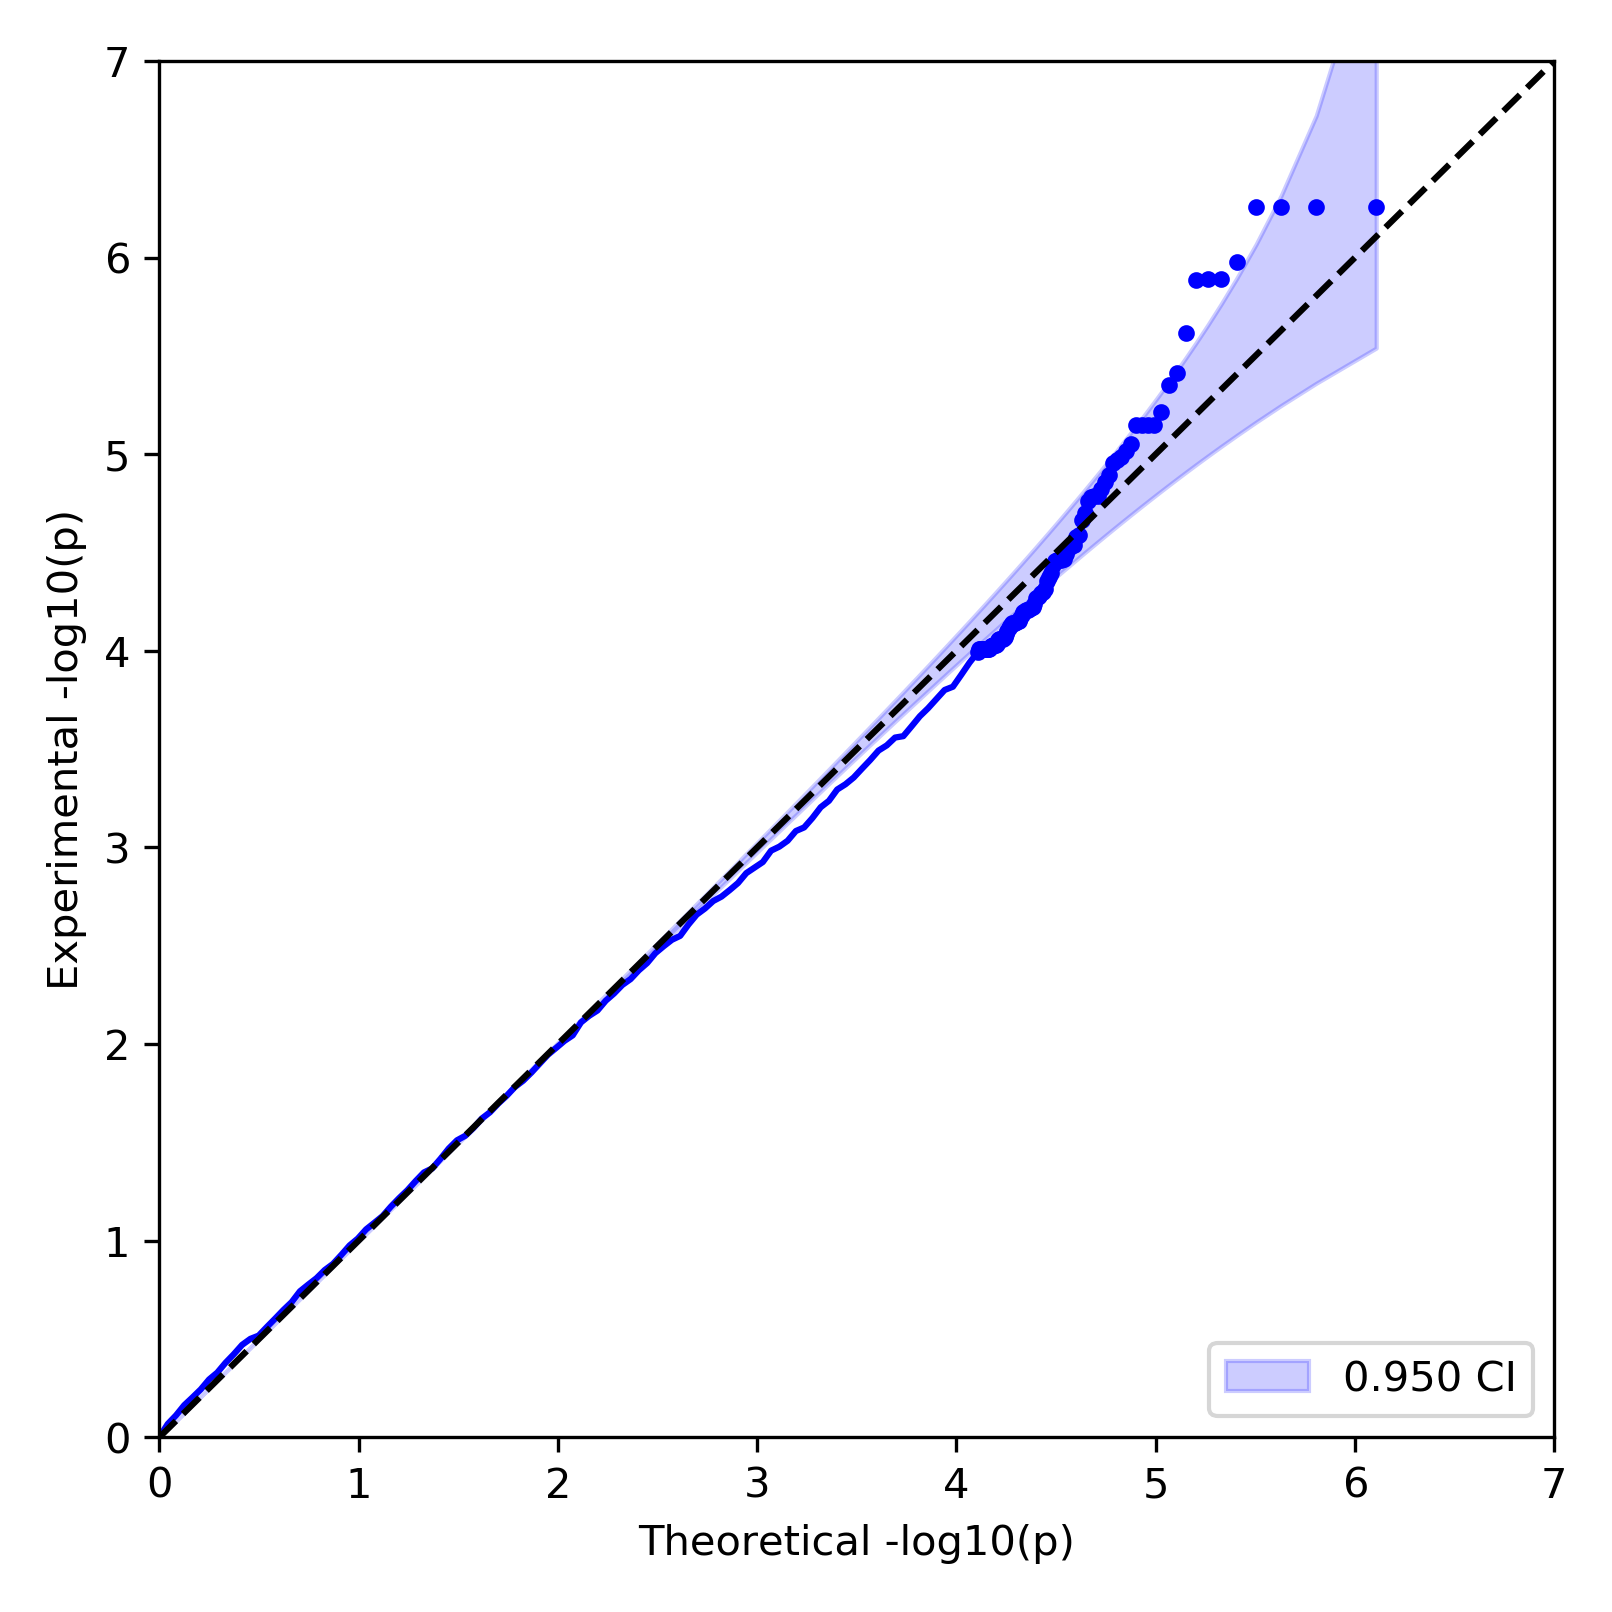
\includegraphics[scale=0.5]{img/qq_plot.png}
    \caption{Manhattan plot and quantile-quantile plot for multiple Testing using 100 000 maxT Permutations}
    \label{fig:1000Permutations}
\end{figure}

The qqplot shows the departure of the upper tail of the distribution from the expected trend along the diagonal is due to the presence of substantially more large test statistic values than would be expected if all null hypotheses were true.The graph suggests that it is unlikely that all the null hypotheses are true. For future study, a list of all SNPs that support the alternate hypothesis should be extracted. Note that no results were available for a million permutations due to memory error.

\subsection{Computational Analysis}
The performance of the entire pipeline including the maxT permutation was measured by collecting data on the Pipeline Duration in seconds and the CPU hours for different permutations. The configuration for these tests were kept constant at 8GB RAM, 4 CPUs and up-to a maximum of 100 parallel tasks.

\begin{table}[h!]
\centering
\begin{tabular}{|l|l|l|} 
\hline
Permutation & Duration (s) & CPU Hours          \\ 
\hline
1           & 96           & 0.1                \\ 
\hline
10          & 109          & 0.1                \\ 
\hline
100         & 91           & 0.1                \\ 
\hline
1000        & 86           & 0.1                \\ 
\hline
10 000      & 158          & 0.6                \\ 
\hline
100 000     & 151          & 2.6                \\ 
\hline
1 000 000   & \multicolumn{2}{l|}{ No Results}  \\
\hline
\end{tabular}
\caption{Performance evaluation for fixed process configuration}
\end{table}

\newpage

\bibliographystyle{unsrt}
\bibliography{bibliography}

\end{document}